% Paper 3, the click model: a new paper on the click model only (the owner's
% decision of 2026-09-20; PLAN.md). Every number of a run is the experiments
% register's (docs/EXPERIMENTS.md, series L, the source fingerprint
% ff5c382d672f); the figures are drawn by figures.py from figures/summary.json,
% the runs reproduced on the merged tree d2064195 (fingerprint 731d0f56c9f9,
% every integer equal); NUMBERS.md maps each number to its source.
\documentclass[11pt]{article}
\usepackage[margin=1in]{geometry}
\usepackage{amsmath,amssymb,amsthm}
\usepackage{booktabs}
\usepackage{graphicx}
\usepackage{hyperref}
\usepackage{caption}
\usepackage{float}
\hypersetup{colorlinks=true,linkcolor=blue,citecolor=blue,urlcolor=blue}
\newtheorem{theorem}{Theorem}
\newtheorem{lemma}{Lemma}
\theoremstyle{definition}
\newtheorem{definition}{Definition}
\newcommand{\Z}{\mathbb{Z}}
\newcommand{\rung}{b}

\title{The click model: an integer GameBoard with one measurement rule,\\
the click that reads one record's squared sum, gives interference,\\
Bell correlations and GHZ, with computed departures from quantum mechanics}
\author{Alon Gonen\\
\small Independent researcher\\
\small \texttt{alon@defounder.ai} \quad ORCID 0009-0008-2701-4599}
\date{September 2026}

\begin{document}
\maketitle

\begin{abstract}
We define an integer model of one quantum in transit with one measurement
rule, and report what it gives when run. Space is a GameBoard of Nodes
joined by six Links; every quantity is a bounded integer; every rule
between births and clicks is local and injective. An event in transit is
a record of rows, each with an amount, an integer phase on a circle of
$N$ steps, a multiplicity and the record's number; a splitter multiplies
a row into rows by integer weights, an exact isometry whose transpose
inverts it; identical rows add and antiphase rows cancel. The one
measurement rule is the click: the apparatus keeps, per record and per
Node, the running sum of the rows' integer phasors; when every row of a
record has ended it lays the cells on a ruler by the squared sums, and a
phase fixed at the birth and read by no rule picks the point; the record
is gathered there and its other rows deleted. That rule is the Born rule,
put in once as inverse-transform sampling of a uniform birth phase;
nothing below the square is derived. From it and the lattice we prove
four theorems (injectivity between clicks given the apparatus's record;
the split an isometry; a pair's marginals exactly $1/2$ at every setting,
no-signalling; the CHSH value at $N$ steps an exact rational within
$8/N + 0.044$ of $2\sqrt2$, on both sides of it) and measure on the
engine, from runs recorded before this text: the Mach-Zehnder always at
one port, Elitzur-Vaidman ($32/17/15$), fringes one quantum at a time,
the pair with cells $27, 5, 5, 27$ at $N = 64$ ($S = 2.75$) and
$S = 181/64$ at $N = 1024$ and $4096$, every marginal exactly one half,
GHZ's exact zeros, a which-path world and a CNOT gate. The click is
non-local: the second click of a pair reads the first's setting and
outcome before it deletes. $S(N)$ lies above $2\sqrt2$ for 252 of the 512
admissible $N$ up to 4096, so a Bell measurement constrains $N$ under
stated assumptions and validates nothing: the photon-pair value
$2.82759 \pm 0.00051$ excludes $N = 64$ and $256$ and admits the powers of
two from 512. Every other statement of the program is listed as a
hypothesis with its status and claimed nowhere.
\end{abstract}

\section{Introduction}

\paragraph{The model in plain words.} The GameBoard is a mail board.
Cells (Nodes), each wired to six neighbours; a wire carries one packet one
step per tick, and nothing travels farther or faster. A packet is four
numbers: how much (the amount), where to (the direction), a rotating
counter (the phase, advanced a fixed step at every wire it crosses) and a
birth number. A cell has no memory: what is in it now is exactly the
packets in it now. The rules are local and few. Transfer: a packet moves
to the neighbour its direction names. Duplication at a splitter: a packet
becomes several packets in several directions with declared shares, the
birth number the same on all. Merging: identical packets add; identical
packets with opposite counters cancel and leave nothing. Deflection
beside a mass: a packet's direction is turned by a table, and the turn
can be undone. The collector, the apparatus, keeps per birth number and
per cell the running sum of the packets' arrows. When every packet of a
birth has ended, the collector lays the cells on a ruler in proportion to
the squared lengths of those sums; a secret number born with the birth,
which no rule ever read, picks the point on the ruler; the whole birth is
recorded at that cell, and the remaining packets of that birth are
deleted wherever they are. For a birth that reaches two collectors, the
collectors' record is one object: the second click reads what the first
wrote, its setting and its outcome, and chooses among what remains. That
read, and the deletion that follows it, are the only action at a
distance in the model; nothing else crosses a wire faster than a packet.
Births happen only at sources, on their own clocks; deaths only at
clicks. Everything between a birth and its click can be run backwards,
given the collectors' record of what they absorbed.

\paragraph{What was asked, and what came before.} The question of this
paper is the one a previous paper on the same simulator asked of four
candidate mechanisms \cite{paper1}: which resource does an integer,
local, causal model need to reproduce the correlations of one quantum and
of a pair. There, every candidate whose information travelled only on
Links stopped at the Bell bound, $S = 2$ exactly, also when the settings
were chosen by events of the GameBoard itself (no superdeterministic
correlation was found), and only a declared shared object, a registry
holding a configured cosine law, reached $2.83$. That framework is the
``before'' of this paper and is not repeated; its engine of the time was
replaced and none of its tables is reproduced. Here the registry and the
configured law are gone. What remains is the lattice, one record with
rows, and one measurement rule, the click of Definition~\ref{def:click}.
Section~\ref{sec:model} defines the model in standard terms; the words
wave, collapse and superposition appear first in Section~\ref{sec:lit},
each as another author's name for one of these things.
Section~\ref{sec:theorems} proves what can be proved of it;
Section~\ref{sec:measure} reports what the engine measured, from runs
recorded before this text was written; Section~\ref{sec:bell} compares
the finite-$N$ Bell value with the experiments; Section~\ref{sec:causal}
places the click in the causal anatomy of Bell's theorem;
Sections~\ref{sec:new} to \ref{sec:hyp} say what is new, what is not
claimed, and what the program hypothesises beside this result. All code,
worlds and recorded runs are archived \cite{zenodo}.

\section{The model}\label{sec:model}

\paragraph{The GameBoard and the circle.} Nodes are the points of a box in
$\Z^3$ (an axis may be periodic); each Node has six Links. Time is the
interval $t \in \Z$. The circle is $\Z_N$ with $4 \mid N$. The tables are
$C_N[p] = \mathrm{round}(256\cos(2\pi p/N))$ and $S_N[p] = C_N[p - N/4]$,
so $C_N[p + N/2] = -C_N[p]$ and $S_N[p + N/4] = C_N[p]$ exactly; the norm
$C_N^2 + S_N^2$ lies in $[65536 - 351,\ 65536 + 361]$ for every power of
two $N \le 65536$ (the extremes $65185$ and $65897$, the latter at
$N = 4096$, $p = 503$: $C = 184$, $S = 179$; at $N = 64$ the range is
$-88$ to $+237$) \cite{checks}. The half-angle tables are $C'_N = C_{2N}$,
$S'_N = S_{2N}$. Directions $D$ are the six headings and declared
primitive integer vectors; the flight table gives, per direction $d$ and
age $\tau$, the Node offset $\mathrm{pos}_d(\tau)$ on the digital line of
$d$, at most one Link per interval and Euclidean speed $1/\sqrt3$ for every
$d$ \cite{beamlaw}.

\begin{definition}[Row and record]\label{def:row}
A \emph{row} is $(x, d, \tau, p, e, h, r, \ell, w, m)$: Node, direction,
age, phase $p \in \Z_N$, emitter, content per unit, record $r$, branch
label $\ell$, amount $w \ge 1$, multiplicity $m \ge 1$. Its amplitude is
\begin{equation}
z = \frac{w}{\sqrt m}\,\frac{C_N[p] + i S_N[p]}{256}, \qquad |z|^2 = \frac{w^2}{m}\cdot\frac{C_N[p]^2 + S_N[p]^2}{65536}.
\end{equation}
Two rows equal in every field but $w$ are one row with the amounts added;
two rows of one record and label equal in every field but a phase
difference of $N/2$ are one row with the amounts subtracted (an equal pair
is no row). The state of record $r$ is an element $\psi_r$ of the free
$\Z$-module $M_r$ on the basis $(x, d, \tau, p \bmod N/2, e, h, \ell, m)$
with $|p + N/2\rangle = -|p\rangle$, taken modulo the scaling
$(w, m) \sim (kw, k^2 m)$; the GameBoard's state is one normal form per
element of $\bigoplus_r M_r$. The norm is $\langle\psi,\psi\rangle =
\sum_{\text{rows}} w^2/m$.
\end{definition}

The host, not any Node, keeps per live record the birth phase $u \in \Z_N$,
the count of live rows, an accumulated pointer $(X, Y)$ per (Node, label)
and a gathered flag. This is the apparatus's layer; the lattice never
reads it.

\begin{definition}[The update rules of one interval]\label{def:rules}
Applied in this order to every row.
\begin{enumerate}
\item[F] Flight: $(x, d, \tau, p) \mapsto (x + \mathrm{pos}_d(\tau+1) -
\mathrm{pos}_d(\tau),\ d,\ \tau + 1,\ p + \varphi)$, $\varphi$ the family's
phase per Link, added only when the step is a Link.
\item[C] Collision and meeting: a permutation of the directions of the
rows at a Node by a fixed table; $r, \ell, m$ unchanged.
\item[S] Split, at a measured event with outputs $\{(d_i, a_i, t_i)\}$,
$a_i \in \Z$: the row $(w, m, p)$ is absorbed and re-emitted as the rows
$(w a_i,\ m A,\ p + t_i)$ on $d_i$ at age $0$, $A = \sum_i a_i^2$. The
balanced splitter is $(1, 1)$, $A = 2$; the reflection's turn is $N/4$.
\item[R] Rotation, at a set with setting $s$, on a label pair $(0,1)$:
$U_s = \begin{pmatrix} C'[s] & S'[s] \\ -S'[s] & C'[s]\end{pmatrix}$, the
rows of label $0$ becoming $(wC'[s], 65536m, p)$ on $0$ and
$(wS'[s], 65536m, p + t)$ on $1$, the rows of label $1$ becoming
$(wS'[s], 65536m, p + N/2)$ on $0$ and $(wC'[s], 65536m, p + t)$ on $1$.
\item[M] Normal form: merge and cancel as in Definition~\ref{def:row}.
\item[B] Birth: a lamp's self-creation at interval $t$ releases record $r$
with $u = t \bmod N$ (the lamp's clock), rows of amount $1$ on its $k$
directions with $m = k$, and, for a pair, the declared labels with integer
weights on separate arms.
\end{enumerate}
\end{definition}

\begin{definition}[The click]\label{def:click}
At a set that reads the sum, the rows of record $r$ and label $\ell$ that
arrive are absorbed and the layer accumulates
\begin{equation}
X \mathrel{+}= \sum 32\,w\,C_N[p + f(\tau, t)],\qquad Y \mathrel{+}= \sum 32\,w\,S_N[p + f(\tau, t)],
\end{equation}
with $f(\tau, t) = \lfloor t n/d\rfloor - \lfloor (t-\tau) n/d\rfloor$ the
family's frequency $[n, d]$ read on the age. The pointer is kept per Node:
interference is coherent within one Node only, and the offer of a set of
Nodes (a detector, a face) and label $\ell$ is the sum over its Nodes of
$(X_x^2 + Y_x^2)/m$, one cell of the ladder, the click landing at the Node
within the set that $u$ selects by the same rungs; all rows at a set share
$m$. When the record's live count reaches $0$, with $T = \sum W$ over its
offers and the cumulative sums $C_1 \le \dots \le C_K = T$ in the declared
order,
\begin{equation}
\rung_k = \left\lfloor \frac{2N C_k + T}{2T} \right\rfloor \quad (\rung_0 = 0,\ \rung_K = N),
\qquad \text{the click is the } k \text{ with } \rung_{k-1} \le u < \rung_k,
\label{eq:rung}
\end{equation}
and the world's list gains one row: the record, $u$, the chosen set and
label, $W$, $T$, the count of combinations before and after. For a record
with arms at two sets $A$ and $B$ (settings $a$, $b$), the first set in
the order takes the coarse rung over its outcomes, and the second the
fine rung within the first's cell with the same $u$, computed from the
joint weights $W(o_A, o_B)$ of Theorem~\ref{th:marginals}; those weights
need $a$, $o_A$ and $b$ together, and the layer, which holds the record,
supplies $a$ and $o_A$ at $B$'s click. The rows not chosen are deleted
lazily, absorbed at their next set and offering nothing.
\end{definition}

\begin{lemma}[One click per record]\label{lem:one}
Every record completes and is gathered exactly once: every row ends at a
set, a face or the border, so the live count reaches $0$; $\rung_K = N$
and $\rung_0 = 0$, so every $u \in \Z_N$ lies in exactly one cell. The
world's row carries the completion interval and the last arrival's
interval; the delay between them is a delay of the record, not of the
lattice.
\end{lemma}

Three things are put in here and not derived, and the paper claims none
of them. Definition~\ref{def:click} \emph{is} the Born rule: the weight is
the squared length of the summed pointer, and the ruler over $u$ is
inverse-transform sampling of a uniform variable, so over births with $u$
uniform on $\Z_N$ the count in channel $k$ is $\rung_k - \rung_{k-1}$, the
nearest integer to $N W_k/T$, Born to the resolution $1/N$. No principle
below the square is offered. The uniformity of $u$ is an assumption about
the source: $u = t \bmod N$ is uniform when the lamp emits at $N$
consecutive intervals, which is how every run below is made (one birth
per $u$), and it is independent of the settings only when nothing that
sets them reads $t \bmod N$, which the choosers' run of \cite{paper1}
measured with settings of odd periods. The tables at $1/256$ are the third
input. What the paper derives is what follows from these with the
lattice's rules: the interference of one record, the exact marginals, the
$\cos^2$ correlation of the pair, GHZ's zeros, and the finite-$N$ value
of $S$. The click is the only step that removes combinations and adds a
row to the world's list; the birth is the only step that adds
combinations. In the engine the law is selected by a world key
(\texttt{amplitude}), and the worlds without it read as before; making
the record form the only click is work in progress and changes nothing
in the runs reported here \cite{beamlaw}.

\section{Four theorems}\label{sec:theorems}

\begin{theorem}[The interval is injective between clicks]\label{th:bijection}
For an interval without a click, $M \circ R \circ S \circ C \circ F$ is an
injective $\Z$-linear map from $\bigoplus_r M_r$ to $\bigoplus_r M_r$
paired with the apparatus's record of the rows the splitters and rotators
absorbed in that interval; the GameBoard's state at any interval between
two clicks, together with that record, determines the state at the birth.
Without the record the split forgets the arriving age.
\end{theorem}
\begin{proof}
$F$ maps a basis element to a basis element and is injective because the
age is kept whole: $(d, \tau) \mapsto (d, \tau+1)$ is injective and the
Node offset is a function of $(d, \tau)$. $C$ is a permutation of the
basis inside its invariant classes by construction of the table. $S$
absorbs the arriving row, whose age, phase and amount are written on the
apparatus's click line, and re-emits at age $0$; given that line it is
injective on the amplitudes by Theorem~\ref{th:isometry}, and without it
two rows differing only in age have the same image. $R$ is injective
because $U_s^{\mathsf T}U_s$ is a nonzero scalar. $M$ replaces a
representative by the normal form of the same element of $M_r$, the
identity on the module. A composition of injective maps is injective. The
engine's inverse interval is the witness on worlds without a measured
event \cite{beamlaw}; with splitters the statement is the algebraic one
with the record.
\end{proof}

\begin{theorem}[The split is an isometry with the transposed inverse]\label{th:isometry}
The split $(w, m) \mapsto ((wa_i)_i, mA)$ preserves $\sum w^2/m$ for every
integer vector $(a_i)$, and the transposed table applied to its outputs,
followed by the normal form, returns the input up to the scaling
$(kw, k^2m)$ with $k = A$. The rotation satisfies $U_s^{\mathsf T} U_s =
n_s I$ exactly with $n_s = C'[s]^2 + S'[s]^2$, and multiplies a record's
norm by $n_s/65536$: an isometry only up to the tables' rounding
($65705/65536$ at $N = 64$, $s = 1$).
\end{theorem}
\begin{proof}
$\sum_i (wa_i)^2/(mA) = w^2 \sum_i a_i^2/(mA) = w^2/m$. The transpose maps
the outputs $(wa_i, mA)$ to $\sum_i a_i (w a_i) = wA$ on the input
direction with multiplicity $mA \cdot A$, that is $(Aw, A^2 m) \sim (w, m)$;
for two inputs at one splitter the cross terms carry phases differing by
$N/2$ (the reflection's two quarter turns) and cancel in the normal form,
which the check with the pairs $(20, 21)$, $(3, 4, 5)$ and $(119, 120,
169)$ confirms integer by integer \cite{design}, and the engine's merge
reproduces on its own rows \cite{beamlaw}. For $U_s$ the diagonal of
$U_s^{\mathsf T}U_s$ is $C'^2 + S'^2$ and the off-diagonal $C'S' - S'C' =
0$ in integers.
\end{proof}

So a record's norm is conserved exactly by $S$ and by the flight, and by
$R$ and by every read through the tables only within the tables' rounding
($-351/65536$ to $+361/65536$ per row for $N \le 65536$); the integer
Mach-Zehnder's total over the 64 birth phases takes eight values from
$65448/65536$ to $65773/65536$, the same eight on every one of its ten
worlds \cite{register}. The normalisation by $T$ in \eqref{eq:rung} makes
the click's probabilities sum to one at completion; it does not restore
the norm along the way, and the paper claims exact unitarity nowhere.

\begin{theorem}[Exact marginals; no-signalling]\label{th:marginals}
For a pair with labels $\{0, 1\}$ of equal weight and settings $a, b$, let
$J(o_A, o_B) = \sum_\ell U_a[o_A][\ell]\,U_b[o_B][\ell]$ and
$W(o_A, o_B) = J^2$. Then the first party's outcome is $+$ exactly for
$u < N/2$ and $-$ for $u \ge N/2$, for every $(a, b)$ and every $N$; and
the second party's count of $+$ is exactly $N/2$ for every $(a, b)$ unless
$2N W(+,+)/T$ is an odd integer (a tie of the rung), in which case it is
$N/2 + 1$. No tie occurs for any setting pair at $N = 8, 16, 24, 32, 48,
64, 96, 128, 192, 256, 512$ \cite{checks}, nor, re-read from the engine's
rows, at $N = 64$, $256$ and $1024$ over all setting pairs and at $4096$
for $a = 0$ and $1024$ \cite{register}.
\end{theorem}
\begin{proof}
Write $n_a = C'[a]^2 + S'[a]^2$. Since the rows of $U_b$ are orthogonal on
the integers, $\sum_{o_B} J(o_A, o_B)^2 = n_a n_b$ for each $o_A$, so
$T = 2n_a n_b$ and the coarse cumulative after the first party's $+$ is
$T/2$: $\rung = \lfloor (NT + T)/(2T)\rfloor = \lfloor (N+1)/2 \rfloor =
N/2$. For the second party, $W(o_A, o_B) = W(-o_A, -o_B)$ (the rows of
$U_s$ are each other's quarter turn), so with $x = N W(+,+)/T$ the counts
are $c_{++} = \lfloor x + \tfrac12\rfloor$ and $c_{-+} = \rung_3 - N/2$ with
$\rung_3 = \lfloor (2N(T - W(+,+)) + T)/(2T)\rfloor = N + \lfloor \tfrac12 -
x\rfloor$. Hence $c_{++} + c_{-+} = N/2 + \lfloor y\rfloor + \lfloor 1 -
y\rfloor$ with $y = x + \tfrac12$, which is $N/2$ when $y \notin \Z$ and
$N/2 + 1$ when $y \in \Z$. The tie condition is $2x \in 2\Z + 1$, that
is $2NW(+,+)/T$ odd. The absence of ties at the listed $N$ is the
computation over every setting pair \cite{checks}.
\end{proof}

The strict-crossing rung $NC_k > uT$ gives the second party $33/64$ in
$3944$ of the $4096$ setting pairs at $N = 64$, a signalling of $1/N$ made
by the rounding \cite{design}; the nearest rung of \eqref{eq:rung} is what
Theorem~\ref{th:marginals} needs. The theorem's scope is what it states:
a pair of two labels with equal weights, the CHSH form, and the rung of
\eqref{eq:rung}; unequal weights and more than two labels are not covered,
and no-signalling for them is open. Where the two settings meet is
explicit in Definition~\ref{def:click}: $B$'s rung is computed from
$W(o_A, o_B)$ with $a$ and $o_A$ supplied by the layer. That the marginal
at $B$ is nevertheless $N/2$ for every $a$ is the content of the theorem;
the joint counts are not local, and the model does not claim they are.

\begin{theorem}[The finite-$N$ Bell value]\label{th:bell}
With the counts of Theorem~\ref{th:marginals},
$E_N(a, b) = 4c_{++}/N - 1$ and
\begin{equation}
\bigl|E_N(a, b) - \cos(2\pi(a-b)/N)\bigr| \le \frac{2}{N} + 4\arcsin\frac{\sqrt2}{512} < \frac{2}{N} + 0.0111,
\label{eq:ebound}
\end{equation}
so at the labels $(0, N/8, N/4, 3N/8)$, $|S(N) - 2\sqrt2| \le 8/N + 0.0443$.
$S(N)$ is an exact rational for each $N$; it lies above $2\sqrt2$ for
$252$ of the $512$ multiples of $8$ up to $4096$ (among them $N = 16, 32$
with $S = 3$ and $N = 128$ with $S = 23/8$) and equals $181/64 =
2.828125$ at every power of two from $512$ through $4096$ \cite{checks}.
\end{theorem}
\begin{proof}
$c_{++} = \lfloor x + \tfrac12\rfloor$ with $x = NW(+,+)/T$ gives
$|c_{++} - x| \le \tfrac12$ and $E_N = 4c_{++}/N - 1$ from the mirror
symmetry, so $|E_N - (4W(+,+)/T - 1)| \le 2/N$. The vector
$(C'[s], S'[s])$ differs from $256(\cos\theta_s, \sin\theta_s)$,
$\theta_s = \pi s/N$, by at most $\tfrac12$ per component, so its
direction differs from $\theta_s$ by at most $\delta = \arcsin(\sqrt2/512)$;
$J(+,+)/\sqrt{n_a n_b}$ is the cosine of the angle between the two
directions, $\cos(\theta_a - \theta_b + \epsilon)$ with $|\epsilon| \le
2\delta$, and $4W(+,+)/T - 1 = 2\cos^2(\cdot) - 1 = \cos(2(\theta_a -
\theta_b) + 2\epsilon)$, within $4\delta$ of $\cos(2\pi(a-b)/N)$. The
four settings add the bounds. The values of $S(N)$ are the computation
from these formulas with the repository's tables \cite{checks}, which
reproduces the design's $176/64$, $720/256$ and $2896/1024$ at $N = 64,
256, 1024$ and the engine's three values below.
\end{proof}

What Theorem~\ref{th:bell} does not say: that $S(N) \le 2\sqrt2$, which is
false for about half the $N$; nor that the deficit is $O(1/N)$ from below,
which holds at the three $N$ the engine ran and not in general. The
tables' term in \eqref{eq:ebound} does not shrink with $N$; it is the
resolution $1/256$ of the circle's tables. At the CHSH labels the tables'
entries are the same at every $N$ ($237, 98$ and $181, 181$), so
$E(0, N/8) = 46565/65773$ and $E(N/4, N/8) = 46437/65773$ exactly at every
$N$ before the rounding of the cells, which is why the powers of two from
512 all give $181/64$ \cite{register}.

\section{The measurements}\label{sec:measure}

Every run of this section is recorded in the experiments register of the
archived code as series L, with its world file, its expectation written
before the run and the source fingerprint \texttt{ff5c382d672f}
\cite{register}; the figures were drawn from the same worlds run again on
the merged tree (fingerprint \texttt{731d0f56c9f9}), every integer equal.
Each world is run for one birth per birth phase, $u = 0, \dots, N-1$, and
the reading tool of the archive replays each run's register through the
layer and equals the run's world list on every run. Every number below
is a count of clicks (a detector reading); the rows' bookkeeping is the
GameBoard's and is reported where it explains a count.

\begin{table}[H]\centering\small
\begin{tabular}{llll}
\toprule
World & Reading & Registered & Expected before the run\\
\midrule
Mach-Zehnder, equal arms, $(20, 21)$ & D1 / D2 over 64 births & $64 / 0$ & $64 / 0$ (offers $1681/1682$, $1/1682$)\\
half turn on arm 2 & & $0 / 64$ & $0 / 64$\\
quarter turn on arm 2 & & $32 / 32$ & $32 / 32$\\
the balanced $(1, 1)$ split & & $64 / 0$ & $64 / 0$; D2's rows cancel on the GameBoard\\
the $(3, 4)$ split & & $63 / 1$ & $63 / 1$ ($u = 63$ falls in D2)\\
arm 2 two intervals longer, $f = 0, 8, 16$ & & $64/0,\ 32/32,\ 0/64$ & the same\\
Elitzur-Vaidman, $(20, 21)$; $(119, 120)$ & absorber / D1 / D2 & $32/17/15$; $32/16/16$ & the same\\
Two slits, one birth at a time & wall / screen / faces of 64 & $34 / 15 / 15$ & the same, every one of 80 sets\\
The pair, $N = 64$, CHSH labels & cells $++, +-, -+, --$ & $27, 5, 5, 27$ ($E = \pm 44/64$) & the same; $S = 176/64$\\
every marginal, all 4096 setting pairs & first party $+$; second party $+$ & $32/64$; $32/64$ & Theorem~\ref{th:marginals}\\
the choosers' 15 setting pairs & $E \times 64$ & $44, -60, 20, 60, -8, -48, -8, 60, -52, -64, 40, 20, -28, -36, 64$ & the same\\
which-path read on one arm & $E \times 64$ & $44, -44, 0, 0$; $S = 88/64$ & the same\\
no maintenance, 116 Links farther & $E(16, 24) \times 64$ & $44$ ($0$ with the read) & the same\\
GHZ, XXX & the allowed triples & $+++, +--, -+-, --+$, 16 each; product $+1$ & the same, the other four exactly 0\\
GHZ, XYY, YXY, YYX & & $++-, +-+, -++, ---$, 16 each; product $-1$ & the same\\
CNOT on $H|0\rangle|0\rangle$, then the pair & $S$ & $176/64$ & the same; CNOT twice the identity\\
the register's ceiling & label rotations on one path & three fit, four refused at load & the same\\
The pair, $N = 1024$ & $E \times 1024$; $S$ & $724, -724, 724, 724$; $2896/1024$ & the same\\
The pair, $N = 4096$ & $E \times 4096$; $S$ & $2900, -2900, 2892, 2892$; $11584/4096$ & the same\\
\bottomrule
\end{tabular}
\caption{The measurements of series L. Every row is a count of clicks over one birth per birth phase; the last column is the expectation written into the worlds' expectation file before the run, from the design's check scripts.}
\label{tab:measure}
\end{table}

\begin{figure}[H]\centering
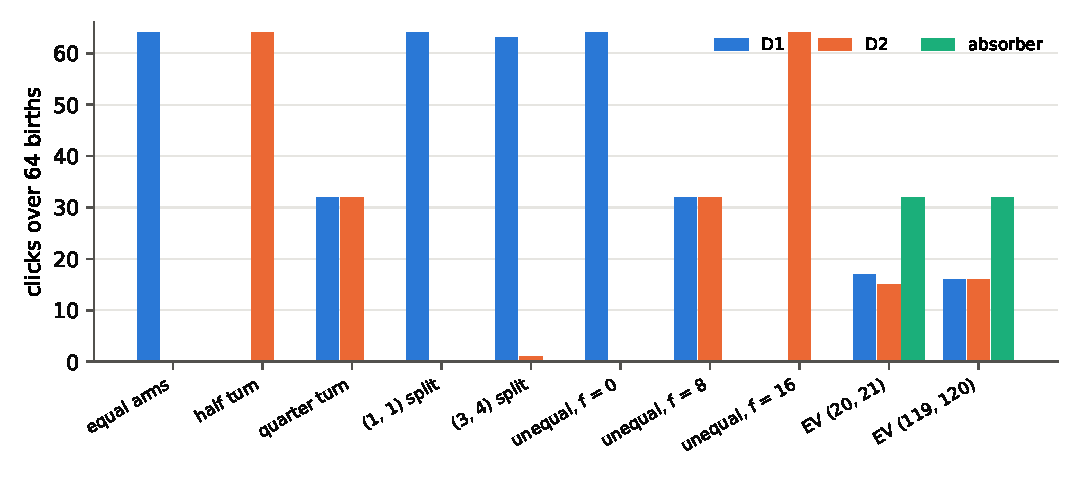
\includegraphics[width=0.95\linewidth]{figures/mach_zehnder.pdf}
\caption{The integer Mach-Zehnder and Elitzur-Vaidman: clicks per port over the 64 birth phases for the ten worlds of L1. Every birth clicks once; the bright port takes every click at equal arms, the dark port at a half turn, and the two split $32/32$ at a quarter turn or at a delay of two intervals at eight phase steps per interval.}
\end{figure}

\begin{figure}[H]\centering
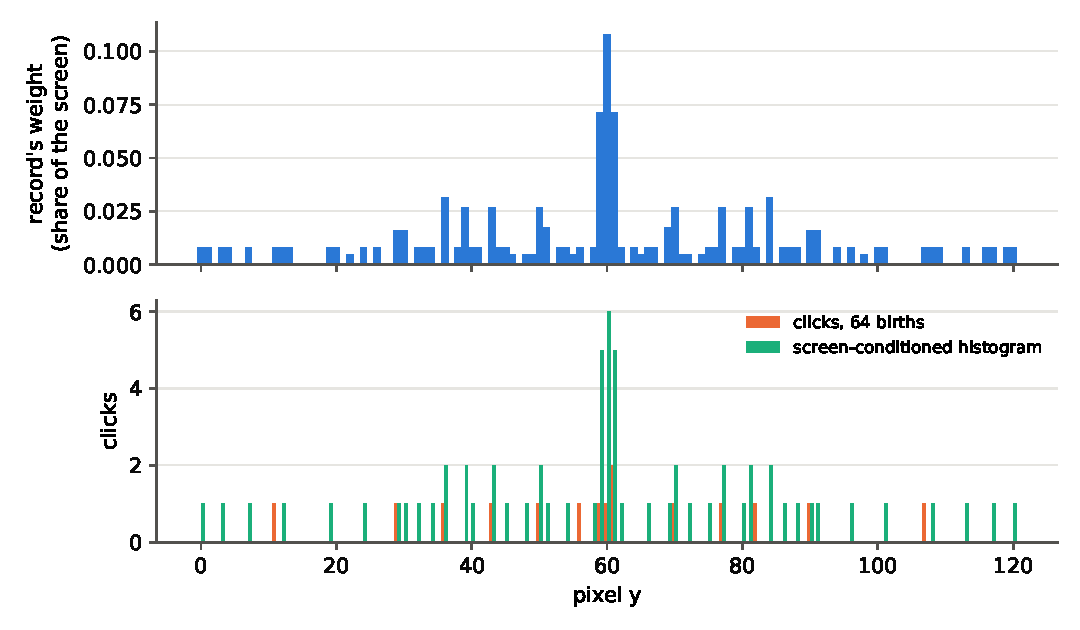
\includegraphics[width=0.95\linewidth]{figures/two_slits.pdf}
\caption{One quantum at a time on the two-slit world of L2. Top: the record's weight per pixel of the screen (the ruler's cells, the same for every birth up to the tables' rounding). Bottom: the clicks that fell on the screen over 64 births, and the screen-conditioned histogram of the generator's reading; the correlation of the histogram with the weights is $0.931$, of the weights with the incoherent sum of the paths $0.744$. The fans are sparse and the pattern is the fans' spots, not a smooth fringe; what the figure shows is that one record's clicks follow its own squared sums.}
\end{figure}

\begin{figure}[H]\centering
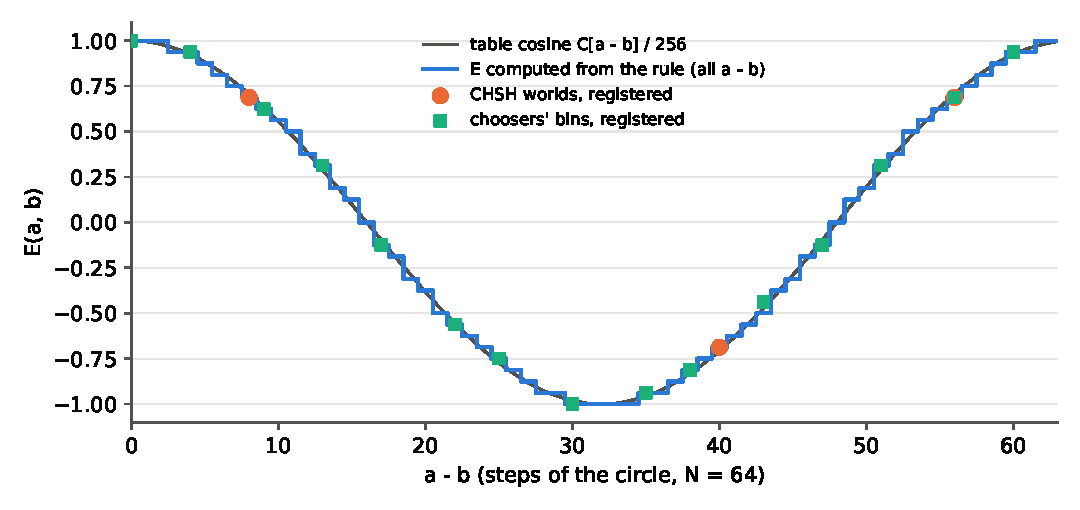
\includegraphics[width=0.95\linewidth]{figures/pair_64.pdf}
\caption{The pair at $N = 64$: $E(a, b)$ against $a - b$. The step curve is $E$ computed from the rule for every setting difference (a computation from the formulas, not a run); the grey line is the tables' cosine; the circles are the four CHSH worlds and the squares the fifteen bins of the choosers' world, both registered runs. Every marginal in every bin is $32/64$.}
\end{figure}

\begin{figure}[H]\centering
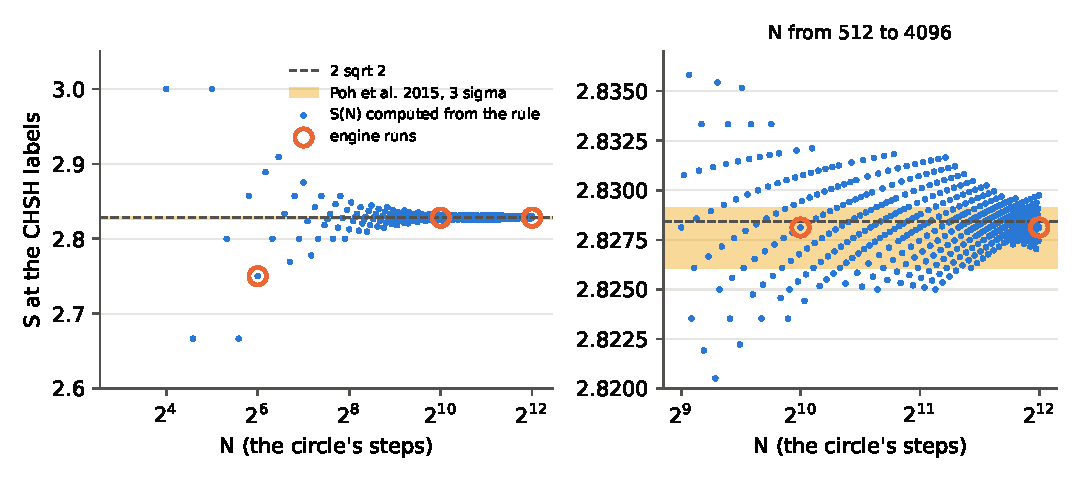
\includegraphics[width=0.95\linewidth]{figures/s_of_n.pdf}
\caption{$S(N)$ at the CHSH labels for every multiple of 8 up to 4096, computed from the rule; the open circles are the engine's runs at $N = 64$, $1024$ and $4096$; the dashed line is $2\sqrt2$ and the band the photon-pair measurement of \cite{poh2015} at three standard deviations. Left: every $N$; right: $N$ from 512 to 4096.}
\label{fig:sofn}
\end{figure}

Three departures from the design's expectations were recorded and not
moved. The record's total over $u$ is not one number but eight, from
$65448/65536$ to $65773/65536$, the tables' rounding depending on $u$;
the rule normalises by the total at completion, so no click moved. The
two-slit world's shares are this geometry's (the wall freed within six
Nodes of each opening so that every fan row leaves the plane; the faces a
third destination) and not the design's $3/5$ and $2/5$; every set's
count equals the reading's. The design's bound $|E - \cos| \le 1/N$ holds
at $N = 1024$ and fails at $64$ and $4096$, as Theorem~\ref{th:bell}
says it must: the cells' grain at $64$, the tables' $1/256$ at $4096$.

\section{The Bell value at finite $N$ and the experiments}\label{sec:bell}

$S(N)$ is a property of the model that nothing in the model fixes: $N$ is
a declared width of the world. The model gives a prediction only once $N$
is chosen, and what a measurement of nature does is constrain $N$, under
two assumptions the paper states and does not defend: that nature's
pairs are this model's pairs at some $N$, and that the experiment's
fair-sampling correction is right. Under them the photon-pair value
$S = 2.82759 \pm 0.00051$ \cite{poh2015} is incompatible with $N = 64$
(152 standard deviations) and $N = 256$ (30), compatible with the powers
of two from 512 (one standard deviation above), admits its first $N$ at
184, and excludes 136 of the 512 values up to 4096 at five standard
deviations, the largest 3016 \cite{checks}. The loophole-free experiments
\cite{hensen2015,giustina2015,shalm2015} constrain $N$ not at all at
their precision ($S = 2.42 \pm 0.20$ in \cite{hensen2015}). A
no-signalling value above $2\sqrt2$ is not forbidden by no-signalling
\cite{pr1994}; at $N = 16$ and $32$ the model gives $S = 3$ with the
marginals exactly $1/2$. Agreement of one value with one experiment
validates nothing beyond that; a comparison with noise and detector
inefficiency in the model's own terms has not been made, and the model
has no rule that would give it.

\section{The click in the causal anatomy of Bell's theorem}\label{sec:causal}

Write $\lambda$ for what is fixed before the settings, $a, b$ for the
settings, $A, B$ for the outcomes. In the terms of \cite{jarrett1984,shimony1986}
as \cite{paper1} used them: $\lambda$ is $u$ with the record, chosen at
the birth before any setting exists and read by no rule that sets a
setting (measurement independence holds by construction); $A$ is a
function of $(u, a)$ alone, $+$ for $u < N/2$ (parameter independence
holds at $A$, and $A$'s marginal is $1/2$); $B$ is a function of
$(u, a, o_A, b)$ through the fine rung within $A$'s cell: parameter
dependence at $B$, exactly where the bonded pair of \cite{paper1} had
it, and outcome independence in the trivial sense that $B$ is
deterministic given $\lambda$ and both settings. The model is
deterministic, measurement-independent and parameter-dependent, the class
Bell's theorem requires of a deterministic model above the bound
\cite{bell1964,chsh1969}; Theorem~\ref{th:marginals} is what keeps the
dependence from being a signal, as \cite{grw1980} showed of quantum
mechanics. What is new against \cite{paper1} is where the dependence
lives: not in a configured cosine of the two settings held by a registry,
but in the second click reading one record's rows, whose products of the
two rotations' entries give $\cos^2$ by the same arithmetic that gives
one record's fringe. The law is the tables' and the rule's; it was not
written into the pair.

\section{What is new}\label{sec:new}

\begin{itemize}
\item One measurement rule, exact in integers, from which interference,
the pair's correlation with exact marginals, GHZ and the gate follow on
one lattice without a configured correlation law, with the rule's
non-locality stated as a read of one record by two clicks.
\item Four theorems about that rule, with the tie, the tables' rounding
and the apparatus's record in their statements, and one exact table
$S(N)$ that puts the model on both sides of Tsirelson's bound.
\item Runs recorded before the text, one birth per birth phase, replayed
from their own registers by a tool independent of the engine's run, and
the departures from the design's expectations kept as measured.
\end{itemize}

\section{What is not claimed}\label{sec:notclaimed}

\begin{itemize}
\item Not a derivation of the Born rule: the square and the uniform birth
phase are the rule (Section~\ref{sec:model}).
\item Not a local model of the pair: the second click reads the first's
setting and outcome; no-signalling is proved for the equal-weight pair
and open beyond it.
\item Not exact unitarity on the lattice: the tables' norm is within
$-351$ to $+361$ of $65536$ per row, the rotation is an isometry only up
to that, and the record's total over $u$ takes eight values.
\item Not a fixed $N$, hence not a prediction of nature's $S$: a
constraint on $N$ under stated assumptions.
\item Not a continuum limit, not spin or polarization (the labels are
abstract), not bosons or fermions, not Lorentz invariance (one speed for
every direction, no boost), not the classical limit as click density
(proposed, not run), not a treatment of noise or detector inefficiency.
\item Not the engine's default: the law runs under a world key, and
making the record form the only click is work in progress.
\end{itemize}

\section{The hypotheses of the program}\label{sec:hyp}

Everything the program states beside this paper's result is listed here
with its status and claimed nowhere. ``Follows from'' is written only
where the rule it follows from is named; the rest is conjectured within
the same GameBoard and not a consequence of the click. Status: registered
(a run in the archived register with a fingerprint and the verdict
quoted), design (a check script's integers, no run), not run, published.

\paragraph{Consequences of the click model.} Entanglement without
maintenance and its end at any intermediate click (from ``nothing between
the birth and the click removes a combination''; registered: the pair
unchanged with one party 116 Links farther, the correlation gone with a
which-path read). The classical limit as click density (from the click
removing combinations and the birth adding them: a body clicked at every
interval has one path; principle of the program; not run). Delayed
choice and the quantum eraser (from the ruler being read at the record's
completion; not run). Hong-Ou-Mandel (from the merge and cancel of
identical rows of two records at one Node; not run; needs the gate's
meeting). The quantum computer in principle and its two ceilings (from
the gate and the register: $n \times 2^n$ rows per path after $n$
entangling gates; on one path 62 balanced splits, 13 passes of a
$(3, 4, 5)$ splitter, 6 of $(20, 21, 29)$, 3 label rotations fit within
$2^{62}$ and a fourth rotation is refused at load; Grover's six rotations
are exact only on the host's integers; design and registered as far as
the refusal). If the GameBoard is a finite machine this is a hard ceiling
on an entangled register, at a width and depth fixed by the store's
capacity and the register's width and not by any law; nature shows no
such ceiling at the sizes reached, and the model fixes no number until a
capacity is declared a law. The bits a click carries: at most $\log_2 N$
per click, since $u$ takes $N$ values and a cell needs $T/2N$ of the
weight; zero at a distance (Theorem~\ref{th:marginals}); derived from the
ruler, not run against an experiment. The boundary between classical and
quantum is the click: sharp per record (a distinguishing click removes
every other combination at once) and continuous over births by the
density of clicks; a partial which-path device is a different apparatus
and a different world in this model, and its counts are an open problem
of the rule, not a prediction.

\paragraph{Conjectured within the same GameBoard, not consequences of the
click.} The forces as columns of one coupling per unit of content
(registered: Newton's identities, Gauss's law, the third law hold on the
plane exactly; the far field of a six-beam source follows the Node
count); the nucleus (registered: the deuteron bound at one Link, the
strong reading a cut $1/r^2$ with the opposite sign and no Yukawa tail,
the alpha a line and not a square); the weak force (registered: the
neutrino's admitted fraction $w/N$ exactly and flat in energy, the
neutron's decay a step with a line spectrum, a bound neutron later or
never: plain disagreements with nature, kept as the law's limits); light
beside a mass (registered: neither bent nor delayed without a rule that
reads the crowd; under the meeting bent toward the mass with the sign and
the $M/b$ form and a grain $10^4$ times nature's angle, not delayed); the
clock's redshift in a field (registered: the $1/r$ form, a pinned
criterion missed at three radii); the Hubble diagram behind the detector
(registered: linear near, coasting far, nothing accelerates); Bohr's
lines (registered: no orbit closes under whole kicks, the lines not
read); the redshift from delay growth on a closed GameBoard and the
supernova test (published, \cite{paper2}); the masses and charges of the
families as the universe's initialisation, not derivable in this law
(decided on the mathematician's verdict; the binding energy that costs
content an open design); dark matter as a closed dimension, $G$ from the
lattice's width, a moving body's clock (not run). Each is stated in the
archived register in the words of its verdict, and none is cited by the
result of this paper.

\section{Literature and positioning}\label{sec:lit}

The click is a non-local step, forced by Bell's theorem because the
marginals are exact and $S > 2$ \cite{bell1964,chsh1969}; it is
parameter-dependent at fixed $u$ in the sense of the causal anatomy of
\cite{paper1} \cite{jarrett1984,shimony1986}; no-signalling is
Theorem~\ref{th:marginals}, as it is a theorem of quantum mechanics
\cite{grw1980}.

't Hooft's cellular automaton interpretation \cite{thooft2016} keeps
determinism and meets Bell by superdeterminism; here the model is
deterministic given $u$, the settings are GameBoard events measured not
to correlate with the pair \cite{paper1}, and the Bell value is met by an
explicit non-local click. Wolfram's hypergraph rewriting and Gorard's
multiway quantum mechanics \cite{wolfram2020,gorard2020} take the
branches of a multiway system as the superposition and a completion as
the collapse; here one lattice, one record with rows, one click with an
exact integer rule and finite tables whose consequences are computed.
Lattice gases \cite{hpp1976,fhp1986} are exact integer dynamics with the
continuum law in the limit; the GameBoard is of that kind, with the
click's reading of one record added. Quantum cellular automata and
quantum lattice gases \cite{bialynicki1994,meyer1996,arrighi2019} are
local unitary rules on complex amplitudes; here no complex number is on
the lattice, the split is an exact integer isometry, and the tables'
unitarity holds within $361/65536$ and is measured, not assumed. Bohm's
theory and quantum equilibrium \cite{bohm1952,dgz1992} derive Born from a
uniform distribution of the hidden variable over the ensemble; the ruler
over $u$ is the same move, one integer per record with a table for the
guidance, and, like Bohm's, non-local at the pair. Nelson's stochastic
mechanics \cite{nelson1966} is stochastic where nothing here is, once
$u$ is fixed. Objective collapse \cite{grw1986,bassi2013} has real
discrete events with a free rate and length; the click is triggered by
the record's completion at the apparatus and has neither, and nothing
collapses spontaneously (a pair stays entangled without maintenance). In
the classification of ontological models \cite{spekkens2007,hs2010} the
rows' amplitudes and $u$ are ontic, so the model is $\psi$-ontic and, as
such a model must be, non-local. On Tsirelson's bound
\cite{tsirelson1980,pr1994} at finite precision
\cite{bhz2005,meyer1999,kent1999}: Theorem~\ref{th:bell} puts the model's
$S(N)$ on both sides of $2\sqrt2$ with the marginals exact, a
no-signalling box of the Popescu--Rohrlich kind at finite $N$, of a size
a Bell measurement of precision $0.0005$ already constrains
(Section~\ref{sec:bell}). The single-quantum build-up of fringes
\cite{tonomura1989,grangier1986}, GHZ \cite{ghsz1990,mermin1990,pan2000}
and interaction-free measurement \cite{ev1993} are the experiments the
measurements of Section~\ref{sec:measure} are named for; none of them is
reproduced in its own geometry, and the two-slit pattern here is a sparse
fan's spots.

\section*{Reproducibility}
The code, the worlds of series L with their expectation file written
before the runs, the reading tool that replays a run's register into its
world list, the check scripts of the exact computations with their
outputs, the runs' summary and the figure script are archived
\cite{zenodo}; the register entry of series L carries every run's world,
duration and source fingerprint, and a table beside the manuscript maps
each number of this paper to its source. Python 3.14, no floating point in
any physical module; the runs take seconds each and the whole series
under two minutes on four cores. The one departure between the register's
tree and the merged tree the figures were drawn from is the fingerprint;
every integer is equal.

\section*{Use of AI tools}
The simulator's code, the design documents, the check scripts and the
drafts of this manuscript were produced with AI coding agents working
under the author's direction and review; the author verified every
number against the archived runs and is responsible for the whole text.
No AI system is an author. [The tool and version are named here at
submission.]

\begin{thebibliography}{99}
\bibitem{paper1} A. Gonen, A finite-integer causal-GameBoard testbed: which resources reproduce interference, causal collapse and Bell correlations on one GameBoard (2026), arXiv preprint.
\bibitem{paper2} A. Gonen, Redshift from delay growth on a closed integer GameBoard: the law, its kinematic correspondence to a scale factor, and the supernova test (2026), arXiv preprint.
\bibitem{beamlaw} The Beam Law and its implementation notes (note 37, the amplitude law), \texttt{docs/BEAM\_LAW.md} of the archived code \cite{zenodo}.
\bibitem{design} The design of \texttt{amplitude-v1} and its check outputs, \texttt{docs/designs/amplitude-v1/} of the archived code \cite{zenodo}.
\bibitem{register} The experiments register, series L, \texttt{docs/EXPERIMENTS.md} of the archived code \cite{zenodo}, with the worlds \texttt{examples/events/amplitude/}, their \texttt{expectations.json} and the reading tool \texttt{tools/amplitude\_path.py}.
\bibitem{checks} \texttt{paper/click\_model/checks/s\_of\_n.py} and \texttt{which\_path\_window.py} with their outputs, and \texttt{NUMBERS.md}, in the archived code \cite{zenodo}.
\bibitem{bell1964} J. S. Bell, Physics 1, 195 (1964).
\bibitem{chsh1969} J. F. Clauser, M. A. Horne, A. Shimony and R. A. Holt, Phys. Rev. Lett. 23, 880 (1969).
\bibitem{jarrett1984} J. P. Jarrett, No\^us 18, 569 (1984).
\bibitem{shimony1986} A. Shimony, in Quantum Concepts in Space and Time, edited by R. Penrose and C. J. Isham (Oxford, 1986), p. 182.
\bibitem{grw1980} G. C. Ghirardi, A. Rimini and T. Weber, Lett. Nuovo Cimento 27, 293 (1980).
\bibitem{thooft2016} G. 't Hooft, The Cellular Automaton Interpretation of Quantum Mechanics (Springer, 2016).
\bibitem{wolfram2020} S. Wolfram, Complex Systems 29, 107 (2020).
\bibitem{gorard2020} J. Gorard, Complex Systems 29, 537 (2020).
\bibitem{hpp1976} J. Hardy, O. de Pazzis and Y. Pomeau, Phys. Rev. A 13, 1949 (1976).
\bibitem{fhp1986} U. Frisch, B. Hasslacher and Y. Pomeau, Phys. Rev. Lett. 56, 1505 (1986).
\bibitem{bialynicki1994} I. Bialynicki-Birula, Phys. Rev. D 49, 6920 (1994).
\bibitem{meyer1996} D. A. Meyer, J. Stat. Phys. 85, 551 (1996).
\bibitem{arrighi2019} P. Arrighi, Natural Computing 18, 885 (2019).
\bibitem{bohm1952} D. Bohm, Phys. Rev. 85, 166 and 180 (1952).
\bibitem{dgz1992} D. D\"urr, S. Goldstein and N. Zangh\`{\i}, J. Stat. Phys. 67, 843 (1992).
\bibitem{nelson1966} E. Nelson, Phys. Rev. 150, 1079 (1966).
\bibitem{grw1986} G. C. Ghirardi, A. Rimini and T. Weber, Phys. Rev. D 34, 470 (1986).
\bibitem{bassi2013} A. Bassi, K. Lochan, S. Satin, T. P. Singh and H. Ulbricht, Rev. Mod. Phys. 85, 471 (2013).
\bibitem{spekkens2007} R. W. Spekkens, Phys. Rev. A 75, 032110 (2007).
\bibitem{hs2010} N. Harrigan and R. W. Spekkens, Found. Phys. 40, 125 (2010).
\bibitem{tsirelson1980} B. S. Cirel'son, Lett. Math. Phys. 4, 93 (1980).
\bibitem{pr1994} S. Popescu and D. Rohrlich, Found. Phys. 24, 379 (1994).
\bibitem{bhz2005} R. V. Buniy, S. D. H. Hsu and A. Zee, Phys. Lett. B 630, 68 (2005).
\bibitem{meyer1999} D. A. Meyer, Phys. Rev. Lett. 83, 3751 (1999).
\bibitem{kent1999} A. Kent, Phys. Rev. Lett. 83, 3755 (1999).
\bibitem{poh2015} H. S. Poh, S. K. Joshi, A. Cer\`e, A. Cabello and C. Kurtsiefer, Phys. Rev. Lett. 115, 180408 (2015).
\bibitem{hensen2015} B. Hensen et al., Nature 526, 682 (2015).
\bibitem{giustina2015} M. Giustina et al., Phys. Rev. Lett. 115, 250401 (2015).
\bibitem{shalm2015} L. K. Shalm et al., Phys. Rev. Lett. 115, 250402 (2015).
\bibitem{tonomura1989} A. Tonomura, J. Endo, T. Matsuda, T. Kawasaki and H. Ezawa, Am. J. Phys. 57, 117 (1989).
\bibitem{grangier1986} P. Grangier, G. Roger and A. Aspect, Europhys. Lett. 1, 173 (1986).
\bibitem{ghsz1990} D. M. Greenberger, M. A. Horne, A. Shimony and A. Zeilinger, Am. J. Phys. 58, 1131 (1990).
\bibitem{mermin1990} N. D. Mermin, Phys. Rev. Lett. 65, 1838 (1990).
\bibitem{pan2000} J.-W. Pan, D. Bouwmeester, M. Daniell, H. Weinfurter and A. Zeilinger, Nature 403, 515 (2000).
\bibitem{ev1993} A. C. Elitzur and L. Vaidman, Found. Phys. 23, 987 (1993).
\bibitem{zenodo} A. Gonen, Universe24: a discrete simulator of local physical laws (Reality Theory), Zenodo (2026), doi:10.5281/zenodo.22738746 (concept DOI, resolving to the latest version).
\end{thebibliography}

\end{document}
